\documentclass[12pt]{amsart}
\usepackage{geometry}                % See geometry.pdf to learn the layout options. There are lots.
\geometry{letterpaper}                   % ... or a4paper or a5paper or ... 
\usepackage{graphicx}
\usepackage{amssymb}
\usepackage{epstopdf}
\DeclareGraphicsRule{.tif}{png}{.png}{`convert #1 `dirname #1`/`basename #1 .tif`.png}

\usepackage[]{natbib}
\bibstyle{apj}
\usepackage{amssymb}

\usepackage{setspace}  % Needed for Double Spacing
\usepackage[english]{babel}
\usepackage{lipsum}

\DeclareGraphicsRule{.tif}{png}{.png}{`convert #1 `dirname #1`/`basename #1 .tif`.png}

\title{Star formation over cosmological time}

\begin{document}
\maketitle

\doublespacing

\noindent
\textbf{Title of Research Opportunity}: RO 18603: The Nature of Star-forming Galaxies at High Redshift\\
\smallskip
\noindent
\textbf{NASA Center}: Goddard Space Flight Center\\
\smallskip
\noindent
\textbf{NASA Advisor}: Dr. Jane Rigby\\
\smallskip


\section{Statement of problem}

\textbf{Main goal:} To investigate the nature of star-forming galaxies in the
epoch when the most stars in the Universe were formed (redshift 1-3), and how
they compare to star forming galaxies in the local Universe. To
disentangle intrinsic properties of the galaxies from environmental differences
over cosmological time spans. To provide calibration and an astrophysical frame
of interpretation for observations with the future James Webb Space Telescope.

\textbf{Short outline:} We propose a two-pronged project consisting of a
local-Universe and a high-redshift part.  \emph{At low redshifts}, we propose to
combine HST-COS observations of existing samples of local star-forming galaxies
from the Hubble Spectroscopic Legacy Archive. These include, but are not limited
to, samples earlier published in
\cite{Heckman2011,Heckman2015,Alexandroff2015,Henry2015,Wofford2013}. The Hubble
Spectroscopic Legacy Archive contains $\sim 175$ HST-COS galaxy spectra
classified as starburst, star forming or dwarf compact; if between one third and
half of these have appropriate data quality, that will lead to a sample of 60-80
objects, with a minimum of 45 spectra from the samples of
\cite{Heckman2011,Alexandroff2015,Wofford2013,Henry2015,JaskotOey} alone. In
these, we will investigate neutral and ionized ISM and CGM properties like
kinematics and column densities in a uniform way similar to our earlier work on
the Lyman Alpha Reference Sample \citep[LARS, ][]{LARSI,LARSII} presented in
\cite{RiveraThorsen2015} (hereafter RT15) and \cite{RiveraThorsen2017}. This
would expand the parameter space coverage of this work,  dramatically improve
the statistical robustness of conclusions drawn from these investigations about
trends and interconnections of these properties. The increase in sample size
would also allow for more sophisticated ways of looking for multi-parameter
correlations like, clustering analysis etc.

Furthermore, data is currently being acquired with HST of the nearby starburst
ESO 338-04 (SAFE, GO 14806 PI: \"O{}stlin); 2 pointings with STIS and 12 pointings
with COS, covering both hot central star clusters and the outer, diffuse
Ly$\alpha$ halo. Part of my project would be  to complement the statistically
oriented work above with an in-depth tomographic study of the ISM in this, one
of the most complex and puzzling local starburst galaxies.  

\emph{At high redshifts}, we propose an analysis of rest-frame optical and UV
spectra observed with Magellan/MagE and Keck/ESI of 17 lensed, star-forming
galaxies at $1 < z < 3$, the sample called "Project Megasaura" (PI: Dr. Jane
Rigby). The high signal-to-noise ratio of these spectra, and the fact that the
objects are spatially resolved due to lensing, makes them ideal for bridging the
gap between high- and low-redshift samples: They have high enough redshifts for
cosmological evolution to be significant, while being of high enough quality
that detailed analyses of Ly$\alpha$, metal absorption lines, nebular emission
etc., like typically done on local samples, is possible. Thus, a detailed,
multi-parameter characterization is possible of these objects, allowing to
thoroughly evaluate differences and similarities between these and the local
objects. 

Furthermore, the lensed spectra contain a wealth of rest-frame NUV lines,
including the important [C \textsc{iii}] $\lambda 1907$, C\textsc{iii}]
$\lambda$ 1909 doublet. This line is by many
considered the most promising beacon for detecting and determining redshifts of
hot, low-mass galaxies in the neutral Universe beyond $z\gtrsim 6.5$
\citep[e.g.][]{Stark2014,Rigby2015,Jaskot2016}.  At these redshifts, the neutral
gas content of the IGM strongly attenuates Ly$\alpha$, which is the most
important observable feature at lower redshifts. This line is typically not
included in local samples due to the wavelength coverage of the Cosmic Origins
Spectrograph.  The Project Megasaur spectra contain both this line and
Ly$\alpha$, and have high enough S/N to analyze some of the most important
tracers of neutral ISM properties in absorption. The combination of these
features provides a unique opportunity to bridge the knowledge and methodologies
of high and low redshift samples, and to provide important tools for pushing the
boundary for how deep into the Universe's past we can see with future James Webb
observations.


\section{Background and relevance to previous work}

\subsection{Project Megasaura}

Project Megasaura is a sample of 17 star forming galaxies at redshifts between 1
and 3, which are strongly lensed by  foreground galaxies or clusters. The
galaxies have been observed in the optical, NIR and MIR with Magellan/MagE and
Keck/ESI, and imaged by HST and Spitzer. The strong lensing gives an unusually 
fine signal-to-noise, allowing for detailed studies in both emission and
absorption.  In itself, the sample is a unique opportunity to study
star-forming galaxies in the epoch where the majority of stars in the Universe
were formed. However, together with a local sample, it also holds the promise of
disentangling intrinsic, evolutionary changes over cosmic time from changes in
cosmic environment, and help understand star formation, galaxy evolution, and
Ly$\alpha$ transfer and escape both locally and in the early Universe.

\begin{figure}[htbp] %  figure placement: here, top, bottom, or page
   \centering
   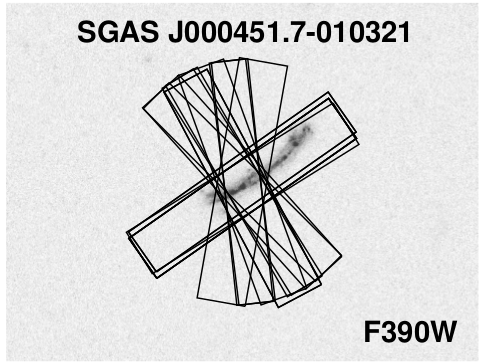
\includegraphics[width=.25\textwidth]{MegasaurExample.png}
   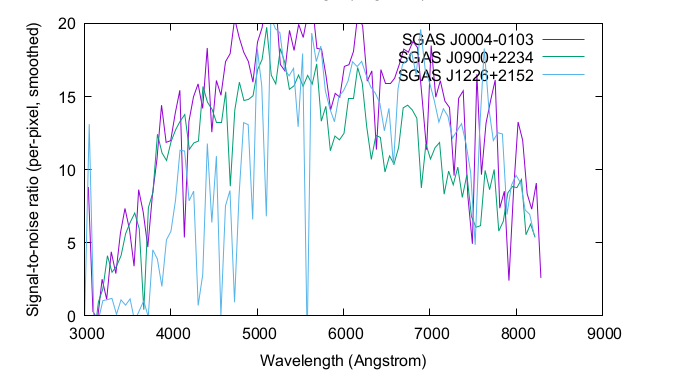
\includegraphics[width=.38\textwidth]{SNRs.png} 
   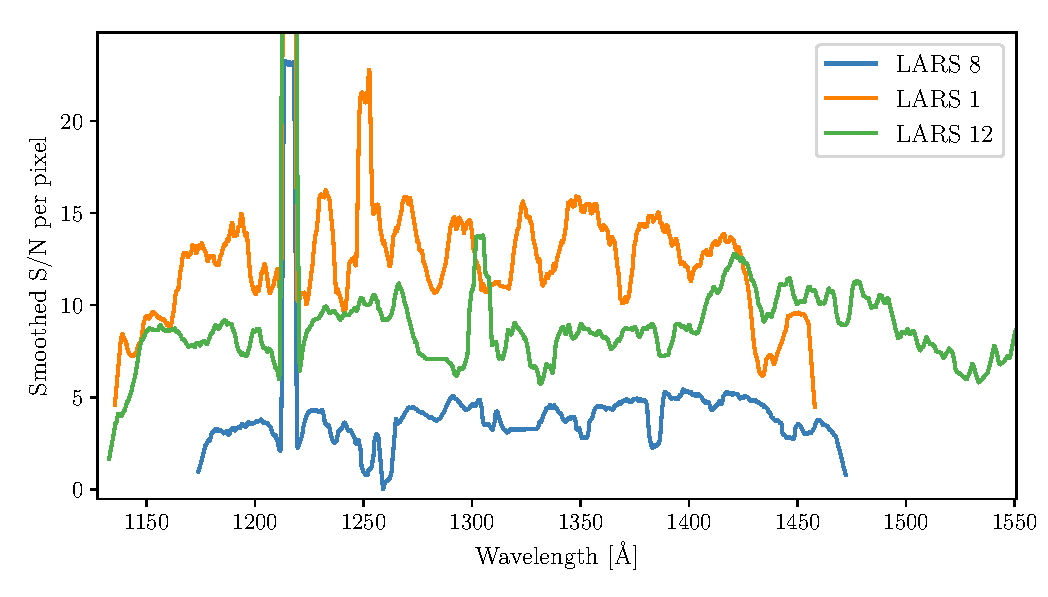
\includegraphics[width=.35\textwidth]{Figures/LARS_SNRs_examples.pdf} 
   \caption{\emph{Left and middle}: Example finding chart for Magellan/MagE
	   observations of a Megasaur galaxy (left), and averaged S/N per pixel
	   in the combined spectra of same galaxy (purple) and two other sample
	   galaxies (right). Images provided by J. Rigby. \emph{Right}: For
	   comparison, S/N for three of the COS spectra of LARS.}
   \label{fig:mega}
\end{figure}

Fig.~\ref{fig:mega} shows an example finding chart of MagE observations of one
of the Megasaura (left), and a curve of running averaged signal/noise per pixel
of this and two other spectra. For comparison is shown S/N of some of the COS
spectra of LARS galaxies of \cite{RiveraThorsen2015}, hinting that the S/N
ratios are cat least comparable. Subsets of the sample have been studied in
depth earlier. Two them are included in \cite{Jones2013}, who performed
studies of neutral kinematics and covering fractions to constrain escape of
ionizing photons, with a large overlap in methodology with
\cite{RiveraThorsen2015,RiveraThorsen2017}. However, these authors did not go
deeper into the Ly$\alpha$/kinematics connection, something we aim to
to do with at least a part of the sample.


Two of the sample galaxies have been subject to in-depth, spatially resolved
studies \citep{Bayliss2014,Bordoloi2016}. \cite{Bayliss2014} compared the
rest-frame NUV emission lines to low-redshifte systems
Galaxies like these have
been studied in smaller numbers by e.g.
\cite{Jones2013,Rigby2014,Rigby2015,Bayliss2014,Bordoloi2016}. \cite{Jones2013}
performed the Apparent Optical Depth analysis to their small sample of lensed
galaxies at redshifts $3 < z < 4$, and found large outflow velocities and low
covering fractions of neutral gas. However, they did not have auxilliary data of
a quality allowing for an accurate comparison with Ly $\alpha$ radiative
transfer models; something we believe possible with the Project Megasaura data. 
\cite{Rigby2014,Rigby2015} focused on near-UV emission and absorption lines of
Mg\textsc{ii}, Fe\textsc{ii}, and C\textsc{iii} in spectrsoscopic samples of
lensed galaxies at redshifts similar to Megasaura, in order , and it is the aim
of this project to be able to analyze these galaxy spectra in ways that will
make them directly comparable to the spectroscopic part of the existing Lyman
Alpha Reference Sample \citep{RiveraThorsen2015} and its extension which is
proposed as another part of this project. 


\subsection{Local-Universe starbursts in the FUV and the Lyman Alpha Reference Sample}

The Lyman Alpha Reference Sample was motivated by the fact that Ly$\alpha$
radiation created in the inner, hot cores of star-forming galaxies and traceable
through H$\alpha$, had been observed to be almost entirely decoupled from the
Ly$\alpha$ emerging from the galaxies. Ly$\alpha$ is subject to strong radiative
transfer effects when  interacting with the neutral ISM on its way out of the
galaxy of origin, and a wide spread of effects like gas column density, dust content,
large-scale outflows, velocity width and more, conspire or compete to either
facilitate or quench Ly$\alpha$ escape.  It was clear that to correctly
interpret the Ly$\alpha$ observations at high redshifts, which potentially hold
the key to a large range of cosmological properties of the Universe, it was
necessary with deep, resolved studies of nearby analogs in order to understand
the processes that govern Ly$\alpha$ transfer and escape. 

\begin{figure}[htbp] %  figure placement: here, top, bottom, or page
   \centering
   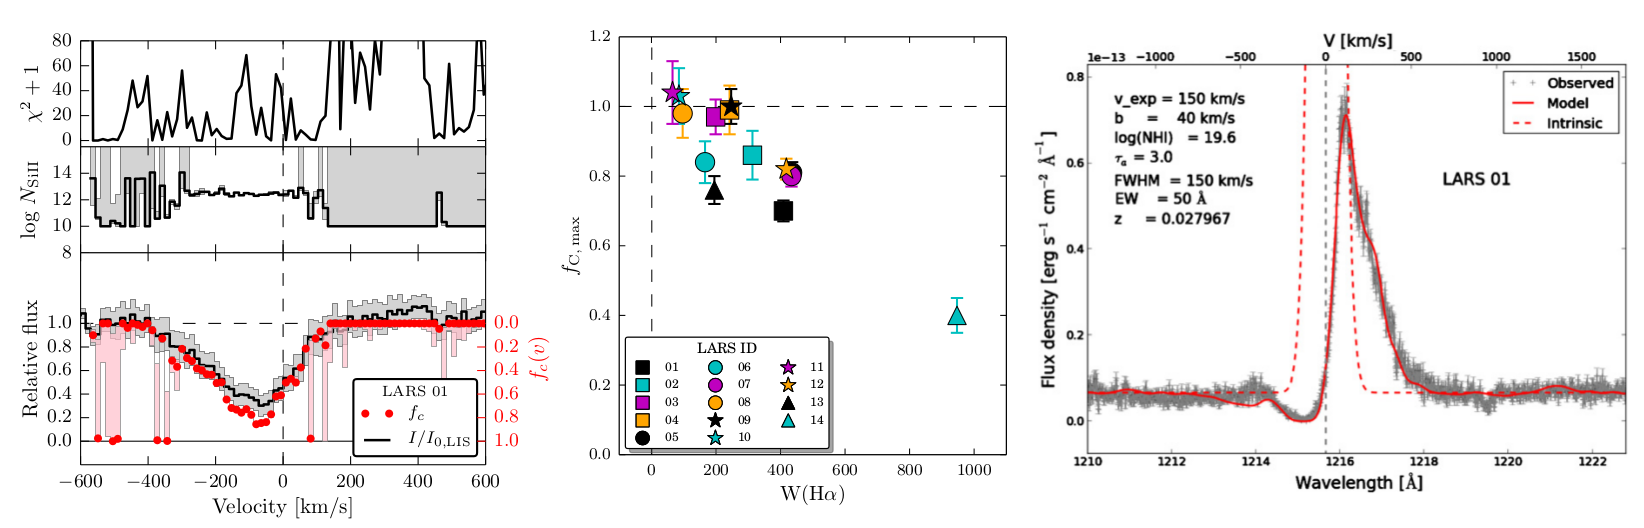
\includegraphics[width=\textwidth]{LarsResults.png} 
   \caption{Left: Result of Apparent Optical Depth analysis of a LARS galaxy.
   Middle panel shows the inferred column densities with errors, lower panel
   shows computed values of $f_C$ (see sect. \ref{sec:weird}), overlaid on the
   averaged LIS metal absorption profile; from RT15. Center: H$\alpha$ EW vs.
   Maximum covering fraction for the LARS galaxies; from RT15. Right: Ly$\alpha$
   profile of LARS 1 (black), with intrinsic Ly$\alpha$ inferred from H$\alpha$
   (dotted red) and the best-fit model from the catalog of the Geneva group
   \citep{Schaerer2011}, from \cite{LARSI}.}
   \label{fig:LARS}
\end{figure}

LARS is a sample of originally 14 galaxies (since extended with 28 more
galaxies, the analysis of which is still ongoing), observed with a large range
of instruments and wavelength ranges, from archival X-Ray data from Chandra and
XMM, to 21 cm eVLA interferometry. The back bone is a set of multi-band HST ACS
and WFC3 imaging and COS spectroscopy. My main contribution to this project has
been the analysis of these COS spectra, published in RT15. Through this work, I
have gained a deep and highly specialized knowledge of the atomic and ionized
ISM in these galaxies, its kinematics and geometry, and its interplay with the
Ly$\alpha$ photons. One of the proposed projects is to run a larger number of
archival COS observations of local star forming galaxies, through the same
machinery as was the LARS, to provide a stronger statistical reliability and a
larger population coverage to the sample, such that a wider variety of
star-forming galaxies at high redshifts have as close and statistically sound
representation in the sample as possible. This would help consolidate our
current knowledge about local Universe conditions, and to draw conclusions about
similarities to and differences from the high redshift Universe with much
stronger confidence.

Fig.~\ref{fig:LARS} shows some core results from LARS in spectroscopy. In the
left panel is the results of AOD computations for one of the galaxies, more
closely explained in the caption. In the middle panel is shown a plot of
EW(H$\alpha$) vs.\ maximum velocity-binned neutral covering fraction in the sample
galaxies (see RT15 for more detail). Here, we found strong correlation,
suggesting that strong SF feedback perforates the surrounding neutral medium,
carving pathways for Ly$\alpha$ to escape. Testing whether this correlation
holds for a larger sample is one of the motivations for the HST Legacy
sub-project. Right panel shows observed Ly$\alpha$ of LARS 1, together the
best-fit model of the Geneva grid, and intrinsic Ly$\alpha$ as traced by
H$\alpha$.  We also propose a similar Ly$\alpha$ profile analysis in this larger
COS Legacy sample and for the Megasaura for which Ly$\alpha$ emission strength
and S/N allows it. 


\subsection{SAFE}

Star forming or starburst galaxies are often messy, strongly interacting systems
with complex kinematics and a strong internal variation in stellar population,
star formation activity etc., as has often been shown in the literature at  low
redshifts; and e.g. \cite{Bayliss2014} show that this can also be the case with
lensed, high-$z$ galaxies. This presents challenges to both observing and
modelling them. 

\begin{figure}[htbp] %  figure placement: here, top, bottom, or page
   \centering
   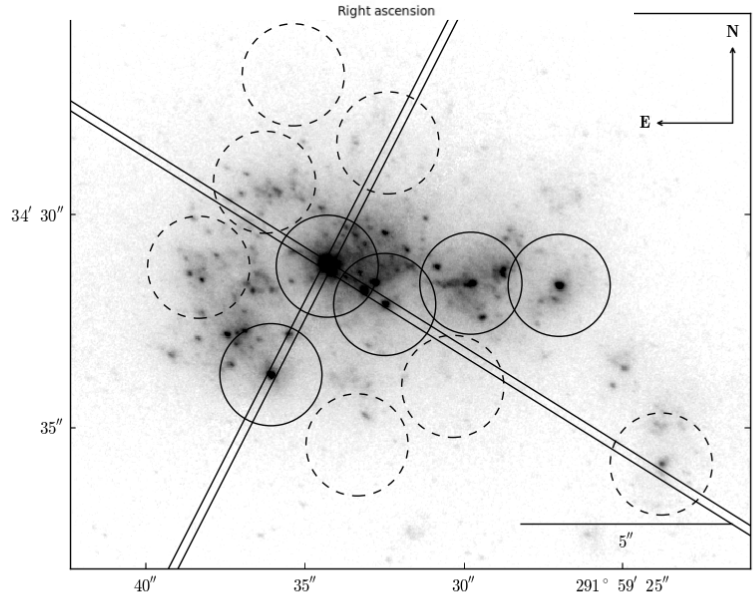
\includegraphics[width=3.5in]{SAFEpointings.png} 
   \caption{STIS and COS pointings for the SAFE project., overlaid on HST UV
   continuum image of ESO 338-04. Image from SAFE proposal by Östlin.}
   \label{fig:example}
\end{figure}

SAFE -- \emph{Star clusters, lyman-Alpha, and Feedback in Eso 338-04} -- is an
attempt to map both star clusters, neutral and ionized ISM, intrinsic and
emerging Ly$\alpha$ and other properties across an entire galaxy in the UV -
something that would normally be done with an IFU in the optical. For lack of
space-borne IFUs, however, this is an attempt to essentially turn the COS into a
coarse-grained one. SAFE will complement the archival COS sample study described
above by giving us a tomographic study of neutral ISM and CGM, Ly$\alpha$
scattering scenarios, etc.

\section{General methodology, procedures to be followed, and timeline for 
completion of each step}

The project is primarily going to rest on spectroscopic observations of
star-forming regions and their surroundings in galaxies at $0 < z < 3$, in
wavelength ranges from the FUV to the MIR, with auxiliary image data included.

This will be complemented with realistic outflow models, stellar population
synthesis like Starburst99 \citep[][and citations therein]{Leitherer2014}, and
photoionization simulation code like \texttt{cloudy} \citep{Ferland2013}, as well
as imaging data, lensing models etc. appropriate for the analysis. 

The spectroscopic work will rest on standard procedures for determination of
e.g. dust content, metal abundances by direct measurements of line strengths and
electron temperature and density \citep[See e.g.][]{Osterbrock}, as well as
empirical, strong line based methods \citep[e.g.][]{YMarino2013}

Methodologies for the specific sub-projects are described in the outline below. 


\subsection{Project outline}

The project for the first two years will fall in four major parts. Two of them
are part of Project Megasaura, two of them focus on local starburst galaxies
as analogs to the Megasaurs.

\begin{description}
	\item[Local starburst galaxies in the FUV] An analysis similar to the 
		one in RT15 of 50-100 starburst and star forming galaxies in the 
		HST-COS Legacy data archives. Systemic redshifts will be 
		determined from SDSS spectroscopy, which will also be used to 
		derive the usual optical emission line-based diagnostics like 
		temperature, ionization, dust content, Oxygen abundance, etc. 
		Metal absorption lines in the COS spectra will be used to
		measure kinematic and, where possible, geometric quantities
		like described in RT15, and Ly$\alpha$, where present in
		emission, will be compared to these findings. Furthermore,
		we have obtained permission to fit the Ly$\alpha$ profiles of 
		both high and low redshift galaxies to the grid of semi 
		analytical Ly$\alpha$ radiation transfer models of
		\cite{Schaerer2011}, and compare to the findings in neutral 
		metal lines. Measurements will, to the extent it is possible, 
		be run in a way directly comparable to the findings of RT15. 
	\item[Megasaura I] This subproject is the first step in the Megasaura 
		work, and contains two steps. \textit{Step 1} will consist in a
		characterization of the star forming knots in the galaxy
		sample: stellar population, dust content, starburst age,
		metallicity from direct methods where applicable, otherwise from
		indirect methods, ionization level etc.; analogous to the 
		properties listed in the first three tables of \citet{LARSI}.
		\textit{Step 2} will be an analysis of ISM kinematics in 
		absorption, looking for outflows etc., and a comparison with
		Lyman $\alpha$ features, to test the known correlations from low
		redshift surveys like LARS. The Megasaur spectra have
		sufficiently high SNR to determine precise zero-point velocities
		from stellar absorption lines, providing a unique opportunity to
		test the findings from low redshifts under early-Universe
		conditions.
	\item[Megasaura II] In this project, we focus on the UV
		emission lines of the lensed galaxies. We can derive kinematic
		properties from NUV Mg\textsc{ii} and Fe\textsc{ii} lines 
		similar to the work of \cite{Bordoloi2016}, using the
		apples-to-apples comparison made possible by Megasaura I and the
		COS Legacy project as a baseline of comparison. Furthermore, the
		properties of Lyman-$\alpha$ emission features and model these
		lines, where applicable, by the outflow and radiative transfer
		model grid of \cite{Schaerer2011}. This would get us one step
		closer to making the Megasaura sample directly comparable to the
		spectroscopic part of LARS and thus provide a bridge from
		the local to the high redshift Universe in terms of star
		formation properties. These lines could also provide us a
		follow-up study to \cite{Rigby2014} on the (non-) correlation of
		Mg\textsc{ii} and Ly$\alpha$ emission in high-redshift
		star forming galaxies; this could triple the sample size for
		these investigations at a low cost due to the measurements
		having already been done in this and earlier papers. 
		Finally, using the above results as a
		starting point would also allow for a deeper study of the
	        properties governing the emission if C\textsc{iii}] 
		$\lambda 1909$, combining an analysis inspired by e.g.
		\cite{Rigby2015} with later photoionization models by
		\cite{Jaskot2016} and earlier found kinematic and physical
		properties of the medium, to help better constrain under which
	        circumstances C\textsc{iii}] is strong and detectable at very
		high redshifts, at which this line and its companion are
		expected to play a crucial role in redshift confirmation of the
		first galaxies with the launch of JWST next year.
		
		% Star-forming galaxies are
		% less well studied in these lines than in the Far-UV; at low
		% redshifts they fall in a range of poor detector coverage of the
		% HST/COS; and at higher redshifts, they are often too faint to be
		% observed in detail with current instruments. With the coming
		% launch of the JWST, however, these lines are going to play an
		% important part in pushing the limits for high-$z$ observations.
		% High-redshift galaxies are typically detected by their Lyman
		% $\alpha$ emission, but at redshifts beyond $z\sim 7$, the
		% neutral fraction of the IGM is high enough
		% to effectively quench the majority of Ly$\alpha$ radiation. The
		% JWST will on the other hand be able to reach much deeper and
		% detect these metallic rest frame NUV lines, like e.g. Mg II, C
	        % III], and Fe II. The combined findings of Megasaura I and the
		% Local HST Legacy Starbursts will provide the foundation to
		% better understand and interpret these lines. 
	\item[SAFE: Star clusters, lyman-Alpha, and Feedback in Eso 338-04] is 
		18 orbits of HST observations of the nearby starburst galaxy ESO
		338-04 being carried out during Cycle 24. The observations
		consist of two STIS pointings centered on the main starburst
		regions and giving very high resolution spectra covering both
		Ly$\alpha$ and H$\beta$, which maps the seed function of
		Ly$\alpha$. On top if this is 12 COS pointing, covering a large
		fraction of the inner parts of the galaxy. About half of these
		are centered on major star-forming regions bright enough to be
		able to measure absorption in the continuum, while the rest
		cover the diffuse Ly$\alpha$ halo and probably mainly will catch
		Ly$\alpha$ and possibly other, faint, line emission. The data
		combined will enable an unprecedented complete mapping of a
		galaxy's ISM in the UV, essentially using COS as a coarse
		grained Integral Field Unit in the UV. The data will allow to
		map both the seeding of Ly$\alpha$, the Ly$\alpha$ that
		eventually escapes, and for large parts the kinematics and
		geometry of the ISM which redistributes it. 
\end{description}

\subsection{Timeline}

\begin{description}
	\item[Months 1-6] Local HST Legacy COS galaxies. Much of the
		computational machinery for this is already in place; so the
		core analysis of this should be relatively straightforward.
		However, some manual work is required for each objects, which of
		course will add up with a sample of an expented $\sim 70$
		galaxies.
	\item[Months 7-16] Megasaura I. This paper will contain a relatively
		large number of measurements and diagnostics, and likely a
		nontrivial amount of data reduction/combination etc., and will
		require a considerable amount of work.
	\item[Months 17-24] Megasaura II. The proportions of the two Megasaura
		papers is uncertain, but a total of 18 months for both seems
		realistic. If the data turn out to merit even more work, it
		should be considered to split it into 3 papers instead.
	\item[Months 25-30] SAFE. This project contains material for large
		amounts of work, but can be split up into smaller parts. A short
                version of a SAFE paper should at least consist of a mapping of 
		the neutral and ionized ISM phases along the line of sight 
		towards the clusters in the relevant pointings, and a 
		characterization of Lyman α in all COS pointings. This will 
		provide a detailed mapping of properties directly comparable to, 
		but more detailed than, the ones known from the Lyman Alpha 
		Reference Sample and from the first projects of this proposal. A
		further elaboration could contain comparisons to detailed
		radiative transfer models, or to spatially resolved Megasaura
		galaxies, if extended Ly$\alpha$ is found int those. 
	\item[Months 30-36] It seems premature to plan this too specifically,
		because the results of the first 2 years' work will probably
		bring up quite a lot of interesting questions and details; but
		one interesting option would be to go in depth with the subset
		of the Megasaura galaxies which are well enough resolved
		spatially to have been observed with multiple pointings.
		Besides, as mentioned above, SAFE will bring very rich data, the
		analysis of which can probably expand well beyond six months.
\end{description}

%  \section{Explanation of new or unusual techniques\label{sec:weird}}
%  
%  The Apparent Optical Depth \citep[AOD,
%  e.g.][]{Savage1991,Pettini2002,Quider2009,Jones2013} method in the
%  implementation we shall use it is not exactly new or unusual, but not widely
%  used in the galaxy community. The method has its name from the depth of an
%  absorption line, in the optically thin regime, simply reflecting the optical
%  depth of the transition along the line of sight to the background source. In its
%  original form \citep{Savage1991}, the idea was to use the relative depths of
%  multiple absorption lines arising from the same ground state of a species,
%  typically Si \textsc{ii}, to unveil hidden saturation in a system.
%  
%  The method can however also be used to determine the column density and covering
%  fraction in a given velocity range in the following way. The 
%  relative residual intensity \(I_{\lambda}\) in a given wavelength interval is: 
%  
%  \begin{equation}
%  	\frac{I}{I_0} = 1 - f_C(1 - e^{-\tau})
%  	\label{AOD1}
%  \end{equation} 
%  
%  \noindent where:
%  
%  \begin{equation}
%  \tau = f\lambda \frac{\pi e^2}{m_e C} N = f\lambda \frac{N}{3.768 \times 10^{14}}
%  \label{AOD2}
%  \end{equation}
%  
%  
%  With multiple value pairs of \(f \lambda\) and \(I/I_0\) arising from a common
%  lower level, it is possible to derive the best-fit values of $f_C$ and \(N\) for
%  gas in the given velocity interval. The method is demonstrated in
%  \cite{Jones2013} and has also been used in \cite{RiveraThorsen2015}, and in
%  Puschnig et al. 2017 (submitted), and \cite{RiveraThorsen2017}.
%  
%  
%  \begin{figure}[htbp] %  figure placement: here, top, bottom, or page
%     \centering
%     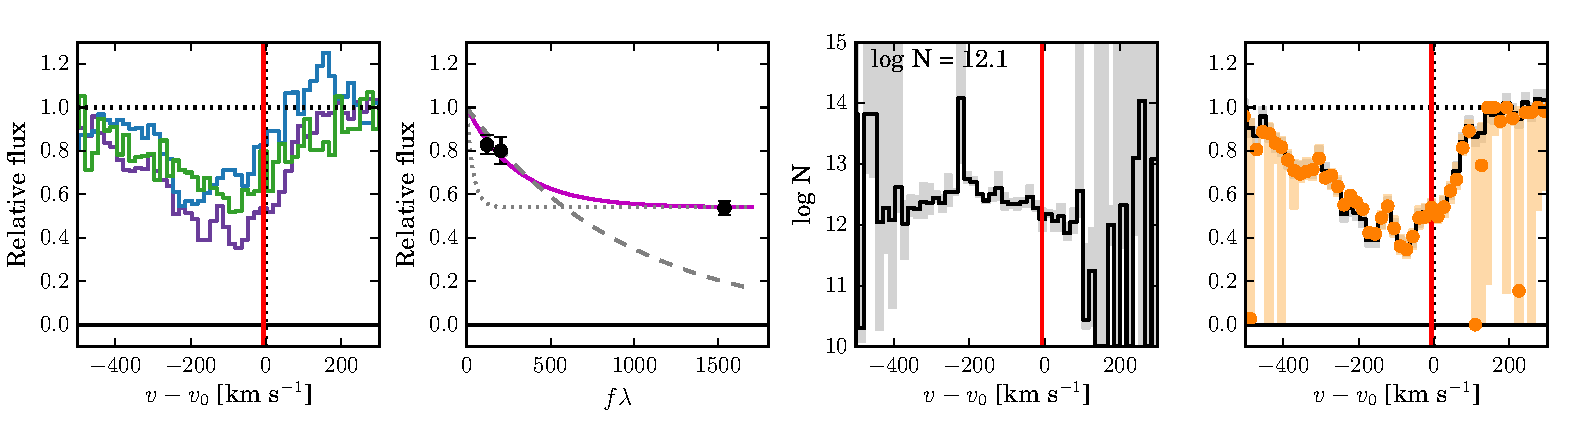
\includegraphics[width=\textwidth]{./AOD-details-example-4pane.pdf} 
%     \caption{Illustration of the AOD method with example data from Haro 11.
%     \textbf{Far left}: Line profile of Si\textsc{ii}\(\lambda\lambda 1260, 1304,
%     1526\), and a vertical red line denoting the velocity bin of interest for the
%     example. \textbf{Center left}: Residual intensity as a function of
%     \(f\lambda\) for the three lines. The best fit of \(I/I_0(f\lambda)\) is 
%     shown in magenta. In gray is shown for illustration \(I/I_0\) in the extreme
%     cases of \emph{a)} unchanged $f_C$ but much higher $N$ (dotted) or \emph{b)}
%     $f_C=1$ and $N$ 0.5 dex lower. \textbf{Center right}: $\log N$ as function of
%     $v$ for these profiles, and \textbf{far right}: $1-f_C$ as function of v
%     (orange circles) superimposed on the profile of Si \textsc{ii} 1260 (black
%  	   steps). Shaded regions are standard errors. }
%     \label{fig:example}
%  \end{figure}
%  
%  
%  The method is illustrated in the four panels of Fig.~\ref{fig:example}. The far
%  left panel of this figure shows the Si\textsc{ii}  $\lambda\lambda 1260, 1303,
%  1526$ lines plotted together. The vertical red line in the figure shows the bin
%  chosen for this example. The next, central left, panel shows the residual
%  intensities for the three lines in this bin as black dots with error bars, this
%  time plotted not against velocity but oscillator strength $f\lambda $. The
%  best-fit function $I/I_0(f\lambda)$, as defined in eqns.~\ref{AOD1} and
%  \ref{AOD2} is shown as a magenta curve. For illustration purposes, the same
%  function is shown with different parameters in the extreme cases of \emph{a)}
%  unchanged $f_C$ but a much higher column density (gray dots) and \emph{b)} for
%  $f_C = 1$ and $\log N = 11.5$, 0.6 dex lower than the measured value. It is
%  clear that with this combination of lines, $\lambda 1260$ is dominating the
%  covering fraction in each bin, while the depth of the lines at $\lambda\lambda
%  1304, 1526$ dominates the column density.  In the third panel, the inferred
%  logarithmic column densities are shown as black steps, with the confidence
%  intervals (found as described in \citet{RiveraThorsen2015}) in shaded gray.
%  Finally, in the far right panel, the inferred covering fractions for each
%  velocity bin are shown as orange dots with confidence intervals, also found as
%  in RT15, as orange shaded areas.  (in fact what is shown is $1-f_C$, to make it
%  better follow the line profile).  In steps is showed the Si\textsc{ii} 1260 line
%  profile with gray shading marking the data $\pm$ the error spectrum.  As shown
%  by \cite{Prochaska2011} and \cite{Scarlata2015}, radiative transfer effects can
%  also alter the line shapes of resonant metal absorption lines, potentially
%  invalidating this method. We show in the paper where the above data are taken
%  from, that in this case, the effect is insignificant. 
%  
%  % \cite{Prochaska2011} has shown that radiative transfer can, in some
%  % circumstances, reshape and partially refill the absorption trough of a resonant
%  % line; and \cite{Scarlata2015} showed that Si \textsc{ii} $\lambda \lambda
%  % 1190,1193,1260$ in certain circumstances can result in an isotropic, expanding
%  % gas imitating the observational fingerprints of a clumpy medium. In the example
%  % of knot C of Haro 11 depicted in fig. \ref{fig:example}, it was however
%  % possible, with the aid of the fluorescent Si\textsc{ii} 1265 line, to constrain
%  % the worst-case effect of these RT effects to be a few percent in $\lambda 1260$,
%  % which would have required practically absent lines in $\lambda \lambda 1304,1526$
%  % to be consistent with values of $f_C$ significantly lower than the ones
%  % inferred. Complex simulations are needed in order to present a more general
%  % solution to this question. 

\section{Expected results and their significance and application}

\begin{itemize}
\item From the HST-COS Legacy sample paper, we expect to get obtain a 
	homogenized analysis of a large number of starbursts in the nearby 
	Universe, improving statistical significance and a giving a better 
	basis for direct comparison of properties like age, mass, ionization, 
	star formation, ISM kinematics, Ly$\alpha$ escape etc. between samples 
	which have so far been treated differently by various authors.  
	This will enable us to learn 
	more about the star-forming population in the local Universe, and the 
	mechanisms that govern Ly$\alpha$ transfer and escape. Furthermore, it 
	will provide an improved sampling coverage of the population and better 
	statistics, both important for comparisons to and calibrations of 
	High-$z$ observations. This work will make strong use of NASA facilities 
	and foster collaborations with the low-redshift community, specifically 
	the LARS collaboration in Stockholm, Paris, Geneva, and more. 
\item From SAFE, we expect to obtain a map of unprecedented accuracy of the 
	neutral ISM of a strong starburst galaxy, as well as its Ly$\alpha$
	emission profile and seed function. It will give a detailed
	understanding of the interplay of dust, line width, outflow velocity,
	clumps, ionization, and Ly$\alpha$ from direct observations, which
	will directly aid in understanding the observations at high redshifts. 
	Furthermore, it will provide much-needed realistic initial conditions 
	for radiative transfer simulations carried out by theorists in
	Oslo and Geneva, and could foster further collaborations
	with these groups. 
\item From Megasaura I, we expect to obtain a characterization
	of the brightest starburst in the sample galaxies, their stellar
	population age, metal abundances, etc., from well-studied rest-frame UV 
	and optical spectral features. We expect to obtain a detailed mapping
	of ISM kinematics, outflows etc., and be able to test the
	insights obtained from local samples against this sample. 
	It will reveal systematic differences between local and
	high-redshift galaxies and, with the proper preconditions, provide a 
	baseline for interpreting non-lensed observations at similar and higher
	redshifts. 
\item With Megasaura II, we expect to obtain knowledge about stellar winds,
	different ISM phases, and ISM kinematics through the less-studied,
        rest-frame NUV emission lines, in particular C\textsc{III}] 1909, to 
	expand existing single-object analyses to a small sample. The knowledge 
	base collected from the previous projects is expected to help calibrate 
	and guide the interpretation of these lines, in turn laying a solid 
	foundation for future spectroscopic observation campaigns with JWST, 
	which have the potential to dig deep into the early, neutral Universe. 
\end{itemize}


% \section{References/Citations}
%\bibliographystyle{apj}
\bibliographystyle{aasjournal}
\begin{scriptsize}
	\bibliography{thesis}
\end{scriptsize}
\end{document}  
